\documentclass{standalone}
\usepackage{tikz}


\usetikzlibrary{calc}
\usetikzlibrary{angles,quotes} % for pic
\usetikzlibrary{patterns,snakes}
\usetikzlibrary{arrows}
\usetikzlibrary{shapes.geometric, arrows}

\tikzset{
    pics/microph/.style={code={
        \begin{scope}[rotate=0]
        \begin{scope}
            \clip (-.3,-.4) rectangle (1.3,1.5);
            \fill[black, rounded corners=1.5] (-.3,-.4) rectangle (1.3,5.5);
        \end{scope}
        
        \fill[white, rounded corners=1.3] (-.1,0) rectangle (1.1,5.1);
        
        \fill[black, rounded corners=1.1] (0,.2) rectangle (1,5);
        \foreach \pos in {2.5, 2.9, 3.3, 3.7}
            \fill[white, rounded corners=.1] (.35,\pos) rectangle +(.8,.25);
        
        \fill[black] (.4,-.4) rectangle (.6,-1.5);
        \fill[black] (0,-1.5) rectangle (1,-2);
        \end{scope}
    }},
}

\begin{document}


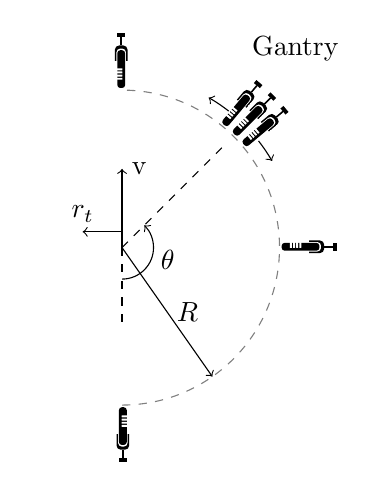
\begin{tikzpicture}
    \def\radius{2cm}
    \def\micSize{0.1}

    %\node[draw, circle, fill=blue!20, minimum size=1cm] at (0, 0) {Center};

    \foreach \i in {0, 130, 135, 140, 90, 180} {
        \path
            (\i-90.9:\radius+15) pic[scale=\micSize, transform shape, rotate=\i] {microph};
    }

    \draw[dashed, gray] (-90:\radius) arc[start angle=-90, end angle=90, radius=\radius];
    
    % prop
    \begin{scope}[rotate=0,  xshift=-0.45cm]
        \draw[scale=1,thick=3, xscale=0.5] node[left=0.5cm] {}
            plot file{../../../app/foils/NACA0012.surf} -- cycle;
    \end{scope}
    \begin{scope}[rotate=180, xshift=-0.45cm]
        \draw[scale=1,thick=3, xscale=0.5] node[left=0.5cm] {}
            plot file{../../../app/foils/NACA0012.surf} -- cycle;
    \end{scope}

    \draw[->] (0,0) -- (0, 1cm) node[right] {v};
    \draw[->] (0,0) -- (-55:\radius) node[midway, right] {$R$};
    \draw[->] (0,0.2) -- (-0.5, 0.2) node[above] {$r_t$};

    \draw[dashed] (0,0) -- (45:0.9*\radius);
    \draw[dashed] (0,0) -- (0, -1);

    \draw[->] (-90:0.2*\radius) arc[start angle=-90, end angle=45, radius=0.2*\radius] node[midway, right] {$\theta$};

    \draw[->] (52:1.1*\radius) arc[start angle=52, end angle=60, radius=1.1*\radius];
    \draw[->] (38:1.1*\radius) arc[start angle=38, end angle=30, radius=1.1*\radius];

    \node at (1.1*\radius, 1.4*\radius) [below] {Gantry};


\end{tikzpicture}

\end{document}